\documentclass{article}

\usepackage[utf8]{inputenc}
\usepackage[T1]{fontenc}
\usepackage[french]{babel}
\usepackage{amsmath}
\usepackage{tikz}
\usepackage{lipsum}
\usepackage[margin=3cm]{geometry}
\usepackage{listings}
\usepackage{csquotes}
\usepackage{subcaption,booktabs}

\NoAutoSpaceBeforeFDP

\usepackage{xcolor}
\usepackage{listings}
\definecolor{dkgreen}{rgb}{0,0.6,0}
\definecolor{ltblue}{rgb}{0,0.4,0.4}
\definecolor{dkviolet}{rgb}{0.3,0,0.5}

% lstlisting coq style (inspired from a file of Assia Mahboubi)
\lstdefinelanguage{Coq}{ 
    % Anything betweeen $ becomes LaTeX math mode
    mathescape=true,
    % Comments may or not include Latex commands
    texcl=false, 
    % Vernacular commands
    morekeywords=[1]{Section, Module, End, Require, Import, Export,
        Variable, Variables, Parameter, Parameters, Axiom, Hypothesis,
        Hypotheses, Notation, Local, Tactic, Reserved, Scope, Open, Close,
        Bind, Delimit, Definition, Let, Ltac, Fixpoint, CoFixpoint, Add,
        Morphism, Relation, Implicit, Arguments, Unset, Contextual,
        Strict, Prenex, Implicits, Inductive, CoInductive, Record,
        Structure, Canonical, Coercion, Context, Class, Global, Instance,
        Program, Infix, Theorem, Lemma, Corollary, Proposition, Fact,
        Remark, Example, Proof, Goal, Save, Qed, Defined, Hint, Resolve,
        Rewrite, View, Search, Show, Print, Printing, All, Eval, Check,
        Projections, inside, outside, Def},
    % Gallina
    morekeywords=[2]{forall, exists, exists2, fun, fix, cofix, struct,
        match, with, end, as, in, return, let, if, is, then, else, for, of,
        nosimpl, when},
    % Sorts
    morekeywords=[3]{Type, Prop, Set, true, false, option},
    % Various tactics, some are std Coq subsumed by ssr, for the manual purpose
    morekeywords=[4]{pose, set, move, case, elim, apply, clear, hnf,
        intro, intros, generalize, rename, pattern, after, destruct,
        induction, using, refine, inversion, injection, rewrite, congr,
        unlock, compute, ring, field, fourier, replace, fold, unfold,
        change, cutrewrite, simpl, have, suff, wlog, suffices, without,
        loss, nat_norm, assert, cut, trivial, revert, bool_congr, nat_congr,
        symmetry, transitivity, auto, split, left, right, autorewrite},
    % Terminators
    morekeywords=[5]{by, done, exact, reflexivity, tauto, romega, omega,
        assumption, solve, contradiction, discriminate},
    % Control
    morekeywords=[6]{do, last, first, try, idtac, repeat},
    % Comments delimiters, we do turn this off for the manual
    morecomment=[s]{(*}{*)},
    % Spaces are not displayed as a special character
    showstringspaces=false,
    % String delimiters
    morestring=[b]",
    morestring=[d],
    % Size of tabulations
    tabsize=3,
    % Enables ASCII chars 128 to 255
    extendedchars=false,
    % Case sensitivity
    sensitive=true,
    % Automatic breaking of long lines
    breaklines=false,
    % Default style fors listings
    basicstyle=\small,
    % Position of captions is bottom
    captionpos=b,
    % flexible columns
    columns=[l]flexible,
    % Style for (listings') identifiers
    identifierstyle={\ttfamily\color{black}},
    % Style for declaration keywords
    keywordstyle=[1]{\ttfamily\color{dkviolet}},
    % Style for gallina keywords
    keywordstyle=[2]{\ttfamily\color{dkgreen}},
    % Style for sorts keywords
    keywordstyle=[3]{\ttfamily\color{ltblue}},
    % Style for tactics keywords
    keywordstyle=[4]{\ttfamily\color{dkblue}},
    % Style for terminators keywords
    keywordstyle=[5]{\ttfamily\color{dkred}},
    %Style for iterators
    %keywordstyle=[6]{\ttfamily\color{dkpink}},
    % Style for strings
    stringstyle=\ttfamily,
    % Style for comments
    commentstyle={\ttfamily\color{dkgreen}},
    %moredelim=**[is][\ttfamily\color{red}]{/&}{&/},
    literate=
    {\\forall}{{\color{dkgreen}{$\forall\;$}}}1
    {\\exists}{{$\exists\;$}}1
    {<-}{{$\leftarrow\;$}}1
    {=>}{{$\Rightarrow\;$}}1
    {==}{{\code{==}\;}}1
    {==>}{{\code{==>}\;}}1
    %    {:>}{{\code{:>}\;}}1
    {->}{{$\rightarrow\;$}}1
    {<->}{{$\leftrightarrow\;$}}1
    {<==}{{$\leq\;$}}1
    {\#}{{$^\star$}}1 
    {\\o}{{$\circ\;$}}1 
    {\@}{{$\cdot$}}1 
    {\/\\}{{$\wedge\;$}}1
    {\\\/}{{$\vee\;$}}1
    {++}{{\code{++}}}1
    {~}{{\ }}1
    {\@\@}{{$@$}}1
    {\\mapsto}{{$\mapsto\;$}}1
    {\\hline}{{\rule{\linewidth}{0.5pt}}}1
    %
}[keywords,comments,strings]




% LTeX: SETTINGS enabled=false

\usepackage{hyperref}
\hypersetup{
    citecolor=black,
    filecolor=black,
    colorlinks=true,
    linkcolor=blue,
    urlcolor=blue
}

\title{Stage L3: Formalisation des dictionnaires en Coq}
\author{Valeran MAYTIE}
\date{Juillet 2023}

% LTeX: SETTINGS enabled=true language=fr

\begin{document}
  \maketitle

  \section{Structure d'accueil}

  Mon stage se déroule au LMF (Laboratoire de Méthodes Formelles)
\footnote{\url{https://lmf.cnrs.fr/}} dans l'équipe Toccata\footnote{
\url{https://toccata.gitlabpages.inria.fr/toccata/index.fr.html}}. C'est une
équipe de recherche du centre Inria Saclay-Île-de-France. Celle-ci est composée
de 7 membres permanents. Parmi eux se trouve Guillaume Melquiond, mon encadrant
de stage. Ses travaux de recherche se situent à l'intersection des domaines de
l'arithmétique des ordinateurs et de la preuve formelle.

  \section{Contexte scientifique}

    \subsection{Présentation Général}

  Coq est un assistant de preuve basé sur de la théorie de types. De ce faite il
possède un langage de programmation qui peut être extrait vers OCaml où
directement interpréter. Le projet ERC Fresco
\footnote{\url{https://fresco.gitlabpages.inria.fr/}} vise à transformer
ce langage en un outil rapide de calcul formel. Un élément clé est la conception
d'un langage de programmation dédié ainsi que des structures de donnée de haut
niveau. Le but de ce stage est de se pencher sur les structures de données
associatives en utilisant les tableaux persistants ajouter en 2010 à Coq.

  Comme Coq possède un langage il est intéressant de chercher des moyens
d'améliorer les performances des structures de données tout en préservant la
validité des preuves. Cela permettrait d'élargir les possibilités d'utilisation
de Coq dans des projets où la performance est critique.

    \subsection{Les enjeux}

  En Coq, la performance a souvent été sacrifiée, les programmes sont souvent
extrait vers OCaml donc il y a peut d'intérêt à créé des structures performantes
directement dans ce langage. Toutefois, de nos jours, Coq est largement répandu
et est utilisé dans des projets qui exploitent directement son interpréteur.
Aujourd'hui les seule structures de dictionnaires disponibles sont les
FMapAVL qui sont difficile à prendre en main et peut performant. Une
implémentation de table de hachage est disponible dans la bibliothèque standard
de Coq, elle à été faite à partir d'arbre de Patricia
\footnote{\url{https://coq.inria.fr/library/Coq.FSets.FMapPositive.html}}
Cependant Une structure de données plus rapide serait bénéfique pour des
opérations telles que la mémoïsation ou le partage maximal
\cite{braibant2014implementing}.

  Il est également très intéressant d'étudier si l'utilisation de structures
impératives persistantes peut améliorer l'efficacité des programmes. En effet,
il n'a pas été mentionné que l'utilisation de structures persistantes augmentera
automatiquement l'efficacité. Il est possible que ces tableaux utilisent
beaucoup de mémoire, ce qui peut entraîner des temps d'allocation plus longs.
De plus, le temps d'exécution du \textit{garbage collector} (ramasse-miettes)
peut également augmenter.

    \newpage
    \subsection{Travail effectué}

Le but du stage est d'explorer différentes implémentations de dictionnaires
basés sur des tableaux en Coq. Le premier travail réalisé a consisté à
comprendre comment les tableaux sont implémentés en Coq en se référant à la
littérature existante \cite{armand2010extending}. Les entiers machines sont
utilisés par les tableaux pour des raisons d'efficacité, il est donc important
de bien comprendre leur fonctionnement. L'implémentation des tableaux utilise
la structure persistante de Baker. Pour approfondir mes connaissances, j'ai lu
l'article de Baker lui-même \cite{baker1991shallow}, ainsi que celui de
Sylvain Conchon et Jean-Christophe Filliâtre \cite{conchon2007persistent}, afin
de compléter le cours donné par Xavier Leroy au Collège de France. 

    \subsubsection{Tables de Hachage}

  Avant de me lancer dans l'implémentation des tables de hachage, j'ai
utilisé des dictionnaires basés sur des arbres de Patricia afin d'avoir une idée
des spécifications des fonctions de base. Ensuite, en me renseignant sur les
différentes implémentations des tables de hachage, j'ai pensé qu'il serait
plus simple de commencer par implémenter les tableaux avec une résolution des
collisions à l'aide de listes chaînées.

  J'ai utilisé les tableaux de Coq pour faire une première implémentation naïf
de table de hachage pour avoir une première base travaille. Pour la résolution
de collision j'ai utiliser des seaux, c'est-à-dire que les case du tableaux sont
composées de liste chainée, donc si deux éléments avec deux clé différentes sont
attribué à la même case alors ils sont tout les deux ajouté à la liste

Ainsi, j'ai défini le type des tables de la manière suivante :

\begin{lstlisting}[language=Coq]
  Inductive bucket : Set :=
    | Empty : bucket
    | Cons (hash: int) (key: A) (value: B) (next: bucket) : bucket.

  Record t : Set := hash_tab {
    size : int;
    hashtab :   PArray.array bucket;
  }.
\end{lstlisting}

  Ensuite, j'ai défini les fonctions de base : \texttt{add}, \texttt{empty},
\texttt{find}. J'ai choisi de faire des tables de hachage similaires à celle
d'OCaml, c'est-à-dire de cacher les anciennes valeur d'une clé à chaque ajout.
\`A cause de ce choix j'ai dût définir une nouvelle fonction \texttt{findall} qui
donne toutes les valeurs associé à la même clé. J'ai donc fait mes premières
preuves sur les tableaux en spécifiant ces fonctions.

\begin{lstlisting}[language=Coq]
  Lemma add_same: forall k (h: t B) v,
    find_all (add h k v) k = v :: (find_all h k).

  Lemma add_diff: forall k k' (h: t B) v,
    k' <> k -> find_all (add h k v) k' = find_all h k'.
\end{lstlisting}

  \subsubsection{Tableaux dynamique}

%   Pour réalisé ces preuves, j'ai dû commencer par créer une version non
% récursive terminale de la fonction \texttt{findall} afin de pouvoir effectuer
% des preuves par le calcul dans Coq, ce qui facilite grandement les démonstrations.
% Ensuite, j'ai rencontré une première difficulté : un utilisateur pourrait
% fournir n'importe quelle table en tant que paramètre, et je n'ai donc
% aucune information sur la valeur par défaut de la table. Deux solutions étaient
% possibles : soit établir un invariant sur la structure de données, soit
% ajouter des conditions dans le programme pour gérer les cas impossibles dans
% les preuves. J'ai choisi la deuxième solution, car la création d'un
% invariant aurait impliqué la création de termes de preuve très complexes, ce
% qui aurait entraîné une perte de la rapidité des entiers machine (il aurait
% souvent fallu passer par des représentations de nombres peu performantes
% dans les preuves).

  Dans un langage impératif pour avoir une table de hachage efficace il faut
utiliser des tableaux dynamique. Je vais donc tester si faire cette
transformation va rendre les tableaux plus efficace.

J'ai décomposé le problème en 3 fonctions :

\begin{itemize}
  \item \texttt{rehash\_bucket}: récupère les élément d'une case pour les mettre
    dans la nouvelle table.
  \item \texttt{copy\_tab}: copie un tableau dans un nouveau tableau.
  \item \texttt{resize}: va redimensionner la table de hachage
\end{itemize}

J'ai spécifié \texttt{resize} avec cette formule

\begin{lstlisting}[language=Coq]
  Lemma find_all_resize:
    forall (h: t) (k: A),
    find_all (resize h) k = find_all h k.
\end{lstlisting}

  Cette spécification a été très difficile à prouver, car \texttt{resize}
utilise deux autres fonctions externe récursive. Pour
commencer, j'ai dû attribuer certaines propriétés aux deux autres
fonctions, qui ont été admise initialement pour m'assurer de leur utilité
par la suite. Une fois que cette étape de preuve a été réussie, j'ai dû
prouver toutes les assertions liées à la fonction en question, parfois sans
disposer de suffisamment d'hypothèses. Pour mener à bien ces preuves, j'ai
également dû ajouter des conditions dans le programme afin de vérifier
si un élément se trouve effectivement dans le bon compartiment (bucket).

      \subsubsection{Tests réalisé}

  Pour pouvoir commencer les tests, j'ai ajouté les fonctions manquantes
telles que \texttt{replace} ou \texttt{mem} \footnote{Hashtable Ocaml.
\url{https://v2.ocaml.org/api/Hashtbl.html}}.
Au départ, j'ai cherché à mettre en place des fonctions qui pourraient
bénéficier d'une optimisation par mémoïsation. J'ai immédiatement pensé à la
fonction de Fibonacci. Cependant, en effectuant cette optimisation, la
complexité devient linéaire et le résultat augmente de manière exponentielle,
ce qui entraîne rapidement des débordement. Les temps d'exécutions ne sont donc
pas représentatifs des performance des dictionnaire.

  Pour régler ce problème j'ai donc cherché une fonction memoïsante plus
difficile à calculer. J'ai donc choisi de faire une fonction qui calcule
les coefficient binomiaux à l'aide du triangle de pascal. Ma fonction a
une complexité de $\mathcal{O}(n^2)$. Pour la memoïsation, j'ai comme type
de clé un couple d'entier et comme valeur un entier. Il faut aussi crée une
fonction de hachage qui éviterai le plus possible les collisions, j'ai
choisi d'utiliser $h(k1, k2)= k1 + k2 \times 345$. Il a fallut aussi faire une
version avec une paire de \textit{positive}\footnote{Représentation d'un nombre
en binaire avec une liste chainée} car les arbres de Patricia vont utiliser ce
type. J'ai utilisé la même fonction puis transformer l'entier
machine en \textit{positive}, cette transformation est de complexité
$\mathcal{O}(\log(n))$ donc un peut couteuse. Il y a donc deux versions du
tests: une avec des clés qui ont une fonction de hachage couteuse et l'autre
avec une fonction de hachage gratuite. J'ai aussi fait le tests avec les
FMap de la bibliothèque standard de Coq\footnote{FMap.
\url{https://coq.inria.fr/library/Coq.FSets.FMapAVL.html}}.

\begin{figure}[ht]
  \centering
  % GNUPLOT: LaTeX picture with Postscript
\begingroup
  \makeatletter
  \providecommand\color[2][]{%
    \GenericError{(gnuplot) \space\space\space\@spaces}{%
      Package color not loaded in conjunction with
      terminal option `colourtext'%
    }{See the gnuplot documentation for explanation.%
    }{Either use 'blacktext' in gnuplot or load the package
      color.sty in LaTeX.}%
    \renewcommand\color[2][]{}%
  }%
  \providecommand\includegraphics[2][]{%
    \GenericError{(gnuplot) \space\space\space\@spaces}{%
      Package graphicx or graphics not loaded%
    }{See the gnuplot documentation for explanation.%
    }{The gnuplot epslatex terminal needs graphicx.sty or graphics.sty.}%
    \renewcommand\includegraphics[2][]{}%
  }%
  \providecommand\rotatebox[2]{#2}%
  \@ifundefined{ifGPcolor}{%
    \newif\ifGPcolor
    \GPcolortrue
  }{}%
  \@ifundefined{ifGPblacktext}{%
    \newif\ifGPblacktext
    \GPblacktexttrue
  }{}%
  % define a \g@addto@macro without @ in the name:
  \let\gplgaddtomacro\g@addto@macro
  % define empty templates for all commands taking text:
  \gdef\gplbacktext{}%
  \gdef\gplfronttext{}%
  \makeatother
  \ifGPblacktext
    % no textcolor at all
    \def\colorrgb#1{}%
    \def\colorgray#1{}%
  \else
    % gray or color?
    \ifGPcolor
      \def\colorrgb#1{\color[rgb]{#1}}%
      \def\colorgray#1{\color[gray]{#1}}%
      \expandafter\def\csname LTw\endcsname{\color{white}}%
      \expandafter\def\csname LTb\endcsname{\color{black}}%
      \expandafter\def\csname LTa\endcsname{\color{black}}%
      \expandafter\def\csname LT0\endcsname{\color[rgb]{1,0,0}}%
      \expandafter\def\csname LT1\endcsname{\color[rgb]{0,1,0}}%
      \expandafter\def\csname LT2\endcsname{\color[rgb]{0,0,1}}%
      \expandafter\def\csname LT3\endcsname{\color[rgb]{1,0,1}}%
      \expandafter\def\csname LT4\endcsname{\color[rgb]{0,1,1}}%
      \expandafter\def\csname LT5\endcsname{\color[rgb]{1,1,0}}%
      \expandafter\def\csname LT6\endcsname{\color[rgb]{0,0,0}}%
      \expandafter\def\csname LT7\endcsname{\color[rgb]{1,0.3,0}}%
      \expandafter\def\csname LT8\endcsname{\color[rgb]{0.5,0.5,0.5}}%
    \else
      % gray
      \def\colorrgb#1{\color{black}}%
      \def\colorgray#1{\color[gray]{#1}}%
      \expandafter\def\csname LTw\endcsname{\color{white}}%
      \expandafter\def\csname LTb\endcsname{\color{black}}%
      \expandafter\def\csname LTa\endcsname{\color{black}}%
      \expandafter\def\csname LT0\endcsname{\color{black}}%
      \expandafter\def\csname LT1\endcsname{\color{black}}%
      \expandafter\def\csname LT2\endcsname{\color{black}}%
      \expandafter\def\csname LT3\endcsname{\color{black}}%
      \expandafter\def\csname LT4\endcsname{\color{black}}%
      \expandafter\def\csname LT5\endcsname{\color{black}}%
      \expandafter\def\csname LT6\endcsname{\color{black}}%
      \expandafter\def\csname LT7\endcsname{\color{black}}%
      \expandafter\def\csname LT8\endcsname{\color{black}}%
    \fi
  \fi
    \setlength{\unitlength}{0.0500bp}%
    \ifx\gptboxheight\undefined%
      \newlength{\gptboxheight}%
      \newlength{\gptboxwidth}%
      \newsavebox{\gptboxtext}%
    \fi%
    \setlength{\fboxrule}{0.5pt}%
    \setlength{\fboxsep}{1pt}%
    \definecolor{tbcol}{rgb}{1,1,1}%
\begin{picture}(7200.00,4320.00)%
    \gplgaddtomacro\gplbacktext{%
      \csname LTb\endcsname%%
      \put(994,767){\makebox(0,0)[r]{\strut{}1e-05}}%
      \csname LTb\endcsname%%
      \put(994,1315){\makebox(0,0)[r]{\strut{}0.0001}}%
      \csname LTb\endcsname%%
      \put(994,1864){\makebox(0,0)[r]{\strut{}0.001}}%
      \csname LTb\endcsname%%
      \put(994,2413){\makebox(0,0)[r]{\strut{}0.01}}%
      \csname LTb\endcsname%%
      \put(994,2962){\makebox(0,0)[r]{\strut{}0.1}}%
      \csname LTb\endcsname%%
      \put(994,3511){\makebox(0,0)[r]{\strut{}1}}%
      \csname LTb\endcsname%%
      \put(994,4060){\makebox(0,0)[r]{\strut{}10}}%
      \csname LTb\endcsname%%
      \put(1095,527){\makebox(0,0){\strut{}$20$}}%
      \csname LTb\endcsname%%
      \put(2836,527){\makebox(0,0){\strut{}$40$}}%
      \csname LTb\endcsname%%
      \put(4576,527){\makebox(0,0){\strut{}$80$}}%
      \csname LTb\endcsname%%
      \put(6317,527){\makebox(0,0){\strut{}$160$}}%
    }%
    \gplgaddtomacro\gplfronttext{%
      \csname LTb\endcsname%%
      \put(195,2413){\rotatebox{-270}{\makebox(0,0){\strut{}temps (s)}}}%
      \csname LTb\endcsname%%
      \put(3986,167){\makebox(0,0){\strut{}n}}%
      \csname LTb\endcsname%%
      \put(6077,2181){\makebox(0,0)[r]{\strut{}$n*n/10000$}}%
      \csname LTb\endcsname%%
      \put(6077,1941){\makebox(0,0)[r]{\strut{}Patricia Nat}}%
      \csname LTb\endcsname%%
      \put(6077,1701){\makebox(0,0)[r]{\strut{}FMap}}%
      \csname LTb\endcsname%%
      \put(6077,1462){\makebox(0,0)[r]{\strut{}Table Nat}}%
      \csname LTb\endcsname%%
      \put(6077,1222){\makebox(0,0)[r]{\strut{}Patricia Int}}%
      \csname LTb\endcsname%%
      \put(6077,982){\makebox(0,0)[r]{\strut{}Table Int}}%
    }%
    \gplbacktext
    \put(0,0){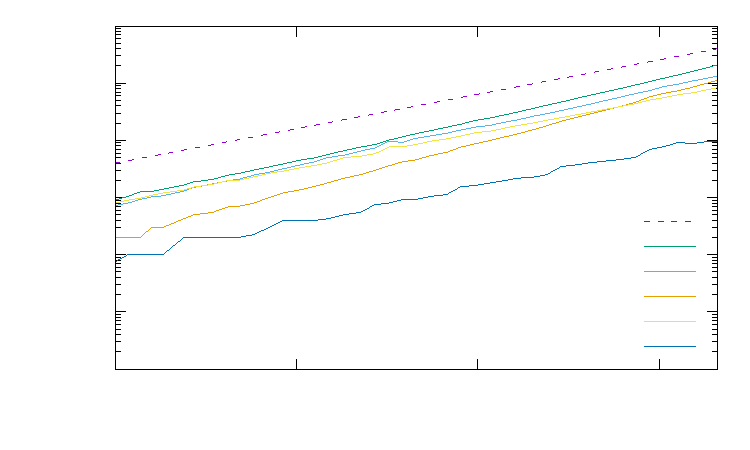
\includegraphics[width={360.00bp},height={216.00bp}]{plot_v1}}%
    \gplfronttext
  \end{picture}%
\endgroup

  \caption{Temps d'exécution de pascal\_memo($2n$, $n$) dans un repère log-log}
  \label{fig:pascal}
\end{figure}

J'ai pût mesurer de très bonnes performances pour les tables de hachage
sur les entiers \hyperref[fig:pascal]{Tableau-1}. Table int et Patricia
représente les deux structure crée avec une fonction de hachage gratuite.
Contrairement à Table Nat et Patricia Nat qui utilise une fonction de hachage
coûteuse.

  J'ai aussi fait une fonction qui vérifie la conjecture de Syracuse
jusqu'à un certain entier $n$. J'utilise des dictionnaires pour retenir les
valeurs déjà croisé, on leur associe l'entier de départ de la suite. Grâce à cet
enregistrement je peux vérifier si j'ai trouvé une boucle (arrêt du
calcul) ou si la valeur à déjà été rencontré (passage à la prochaine valeur).
Les tests de performances ont été effectué avec deux types de valeur numérique :
les entier machines et les \textit{positive}. J'ai testé avec mon implémentation
des arbres de Patricia, nos tables et les FMap de Coq. J'ai aussi utilisé les
PositiveMap\footnote{Patricia. \url{https://coq.inria.fr/library/Coq.FSets.FMapPositive.html}}
de Coq qui sont aussi des arbres de Patricia.

\begin{table}[h!]
  \centering
  \begin{tabular}{c|c c c c c c}
    n & Table Int & Patricia Int & FMap Int & Table Positive & Patricia Positive & PositiveMap \\
    \hline
    100     & 0.003s & 0.005s   & 0.004s  & 0.003s  & 0.003s & 0.002s  \\
    1000    & 0.021s & 0.049s   & 0.044s  & 0.023s  & 0.035s & 0.021s  \\
    1000    & 0.146s & 0.241s   & 0.403s  & 0.191s  & 0.158s & 0.202s  \\
    10000   & 1.243s & 2.44s    & 3.87s   & 1.747s  & 1.794s & 1.5s    \\
    100000  & 13.101s & 29.101s & 48.856s & 18.251s & 19.57s & 16.969s \\
  \end{tabular}
  \caption{Vérification de la conjecture de syracuse de $1$ à $n$}
\end{table}

  Pour la suite du stage il serait utile de faire de nouveaux tests en essayant
de pousser les optimisation des fonctions avec les arbres, par exemple passer
avec les \textit{positive} pour le calcul des coefficient binomiaux. Ensuite il
faudra que je fasse une librairie Coq rendre les tables de hachage utilisables
pour tous.

  \newpage
  \section{Retour d'expérience}

  Ce stage a été une excellente opportunité pour apprendre de nouvelles choses
et approfondir mes connaissances dans certains domaines. J'ai pu réaliser ce
stage grâce au TER que j'ai effectué d'octobre à avril, et qui a été l'un des
<<cours>> les plus utiles pour mener à bien ce stage. En travaillant sur
CompCert, j'ai appris à utiliser Coq, et pour apprendre à réaliser des preuves,
j'ai pu consulter le livre "Coq'Art" de Bertot et Casteran\cite{bertot2015coq},
qui m'a généreusement été prêté par Christine Paulin-Mohring durant le TER et le
début du stage. Le cours de génie logiciel avancé m'a également beaucoup aidé,
car il m'a permis de comprendre l'importance des spécifications et de connaître
les outils disponibles pour vérifier ces propriétés parfois très complexes. Le
cours de lambda calcul a également été très utile pour mieux comprendre ce qui
se passe dans Coq. Il m'a donné des bases solides pour être plus à l'aise lors
de la lecture d'articles, car le lambda calcul est l'un des concepts clés de la
preuve formelle. Les cours de programmation, tels que celui d'algorithmique en
L2 et PFA, m'ont également donné de bonnes bases pour améliorer la qualité de
mon code.

Grâce à ce stage, je suis confiant dans le fait que j'aurai de solides bases
pour intégrer le \textit{Master Parisien de Recherche en Informatique}. Cette
expérience m'a confirmé que les méthodes formelles sont la voie que
je souhaite suivre.

  \section{Remerciement}

  Pour conclure, j'aimerais remercier les personnes qui ont contribué au bon
déroulement de mon stage et du TER. Tout d'abord, je tiens à remercier Sylvain
Conchon pour m'avoir mis en contact avec Guillaume, que je remercie également
pour m'avoir appris tant de choses tout au long de cette année et pour s'être
occupé de moi une journée par semaine pendant un an. Je souhaite également
exprimer ma gratitude envers Jean-Christophe Filliâtre pour m'avoir
généreusement prêté des livres, ce qui a suscité mon intérêt pour la lecture
scientifique. Enfin, je tiens à remercier tous les chercheurs du LMF pour leur
accueil chaleureux.

  Ces personnes ont joué un rôle essentiel dans mon parcours et ont contribué à
rendre cette expérience enrichissante et gratifiante.

  \bibliographystyle{alpha}
  \bibliography{ref}

\end{document}
